\chapter{シミュレーションによる評価} \label{chapter:evaluate}
本章では、提案した手法の評価を行う。
\ref{section:評価方法}節では、評価方法について述べる。
\ref{section:実験条件}節では、シミュレーション実験の条件について述べる。
\ref{section:結果}節では、シミュレーション実験の結果を述べる。
\ref{section:考察}節では、考察について述べる。

%%%%%%%%%%%%%%%%%%%%%%%%%%%%%%%%%%%%%%%%%%%%%%%%%%%%%%%%%%%%%%%%%%%%%%%%%%%%%%%%
\section{評価方法} \label{section:評価方法}
本節では、評価方法について述べる。
まず、評価を行うにあたって、本手法により目指している動作について述べる。
そして、その目指している動作を達成しているかを評価するときの基準について述べる。

%%%%%%%%%%%%%%%%%%%%%%%%%%%%%%%%%%%%%%%%
\subsection{目指している動作}
本論文において、移動ロボットに行わせたい動作は、状態推定の不確かさを考慮した障害物回避の動作である。
通常行われるような、最も確率の高い姿勢を真の姿勢と仮定して行われる行動計画では、確率的な推定の情報が行動に生かされない。
そこで、信念分布内のどこかにロボットが存在する可能性を考慮し、
信念分布を近似するパーティクル全体が、障害物内に入らないような行動を行わせることを目指している。

また、PFC法のゴール探索動作が行われることも求められる。
分布全体を徐々にゴールになぞるように流し込み、分布内に存在するロボットがいずれゴールへと到達する。
これにより、信念分布がゴール範囲よりも大きい場合でも、ロボットがゴールすることを可能にする。

信念分布が大きいときに、この2つの動作をそれぞれ状況にあわせて行うことを目指す。
周囲に障害物があるときには、分布全体が障害物を避けるような動作を行わせる。
そして、ゴール周辺では、停滞することなくゴールへと到達するするために、分布をゴールへと流し込む探索動作を行わせる。

%%%%%%%%%%%%%%%%%%%%%%%%%%%%%%%%%%%%%%%%
\subsection{評価方法}
1回のナビゲーションタスクにおいて、障害物の回避とゴールの探索動作がそれぞれ行えているかを評価する。
タスクは、ロボットがゴールへと到達したときに成功とみなす。
逆に、ロボットが障害物内に侵入した時点で、そのタスクは失敗とする。
ロボットがゴールへ到達するのに300秒以上かかった場合も、同様に失敗とする。

ロボットは初期姿勢の配置と動作モデルは、それぞれノイズを有している。
ロボットの初期姿勢は、正規分布に従うばらつきを有しており、
パーティクルの初期分布も、同様の正規分布に従い配置されるものとする。

また、ロボットの状態推定の不確かさが大きい状況を維持するために、
ロボットが観測により得られる情報が非常に制限されているものとする。
自身の姿勢推定に用いることができる情報は、ゴールしているか否かの情報のみである。
これは、PFC法による行動を行うために必要となる観測情報である。
そのほかの距離センサやランドマークによる観測は行えないものとする。

そのために、ロボットがナビゲーションにおいて、状態推定を考慮した障害物回避とゴールの探索を行えているかを、
\begin{itemize}
  \item タスクの成功率
  \item タスク成功時の平均時間
  \item 障害物内を移動したパーティクル数×時間 の平均
\end{itemize}
の3つを基準に評価する。
この基準をもとに、提案手法を、通常のPFC法、Q-MDP法、ロボットの真の姿勢による最適方策、
そしてパーティクルの平均姿勢による最適方策の4つと比較する。
各手法それぞれの試行を100回行うことで評価する。


%%%%%%%%%%%%%%%%%%%%%%%%%%%%%%%%%%%%%%%%%%%%%%%%%%%%%%%%%%%%%%%%%%%%%%%%%%%%%%%%
\section{シミュレーション実験の条件} \label{section:実験条件}
本節では、シミュレーションによる実験の条件について述べる。
まず、評価を行うための環境について述べる。
そして、ロボットの初期姿勢や状態遷移確率、行動の種類について述べ、また、MCLやその他パラメータについて述べる。

%%%%%%%%%%%%%%%%%%%%%%%%%%%%%%%%%%%%%%%%
\subsection{環境}
二次元のシミュレータを用いて、評価を行う。
評価は、図\ref{fig:environment}に示すように、一つの障害物を有する、幅が$10[\si{m}]$の正方形の空間で行う。
灰色で示された領域は、障害物を意味する。
また、環境の中央を原点とする$X-Y$座標系$\Sigma$を定義する。
$X$軸と$Y$軸はそれぞれ環境の縁と並行に設定されている。
\begin{figure}[tbp]
  \begin{center}
    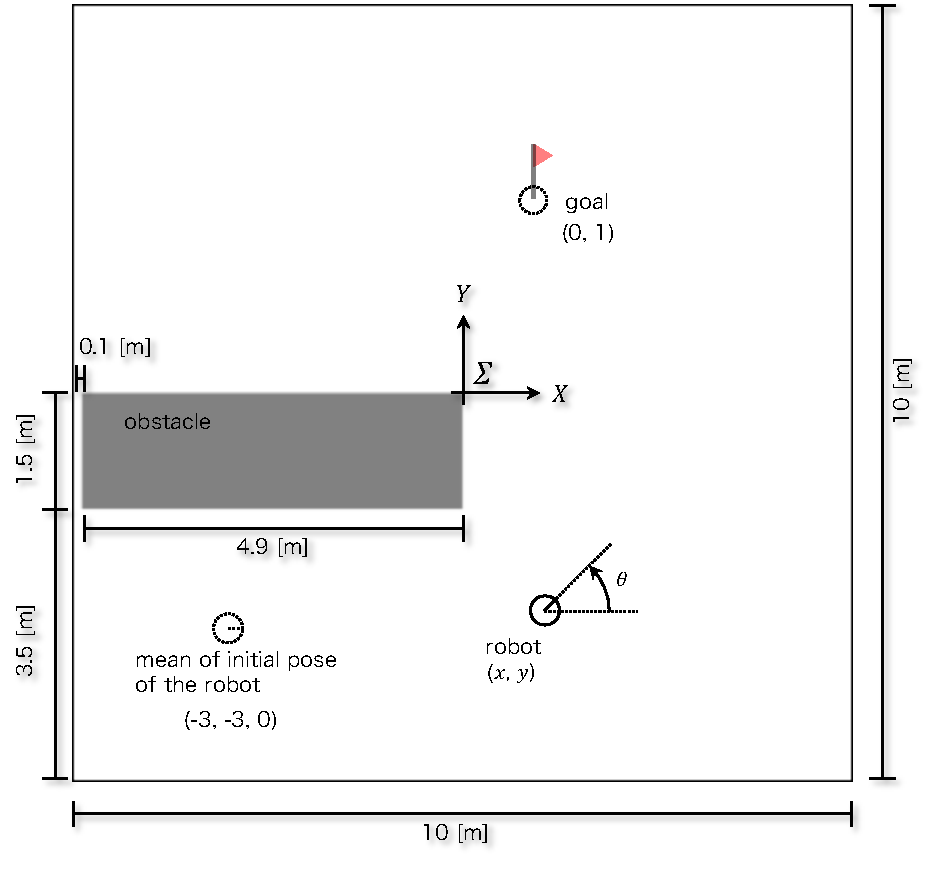
\includegraphics[width=12cm, ]{environment.pdf}
    \caption{Environment map with one obstacle.}
    \label{fig:environment}
  \end{center}
\end{figure}

%%%%%%%%%%%%%%%%%%%%%%%%%%%%%%%%%%%%%%%%
\subsection{ロボットの行動と初期姿勢}
ロボットの行動は、$\mathcal{A} = { fw, ccw, cw }$の3つから選択されるものとする。
行動はそれぞれ、
\begin{itemize}
  \item $fw$: $(0.2 + 0.01\sigma) \si{[m/s]}$ の前進
  \item $ccw$: $(1 + 0.01\sigma) \si{[rad/s]}$ のその場旋回
  \item $cw$: $(-1 + 0.01\sigma) \si{[rad/s]}$ のその場旋回
\end{itemize}
を意味する。
ここで、$\sigma$は正規分布$\mathcal{N}(0, 1)$から生成されるノイズであり、$\sigma \sim \mathcal{{N}}(0, 1)$のように選択される。
ロボットは、この運動モデルを知っていると仮定する。

ロボットの初期姿勢は、
\begin{equation}
\label{robot initial pose}
  (x, y, \theta) = (-3 + 0.3\sigma, -3 + 0.3\sigma, 0.03\sigma)
\end{equation}
のように配置され、各試行ごとに正規分布に従いばらつく。
% 初期配置の例を図に示す。

%%%%%%%%%%%%%%%%%%%%%%%%%%%%%%%%%%%%%%%%
\subsection{価値関数の計算}
価値関数を計算する状態空間$\mathcal{X}$は、二次元の位置$(x, y)$と方向$\theta$の3状態からなる。
計算のための離散化は、位置についての離散状態の幅を$0.05\si{[m]}$とし、方向については$10\si{[deg]}$とする。
図\ref{fig:environment}に示した縦横の幅が$10\si{[m]}$の空間を離散化すると、離散状態は$200 \times 200 \times 36$となる。
この、合計$1,440,000$離散状態の価値関数を事前に計算する。

状態遷移の報酬について設定する。
このタスクでは、ゴールまで早く到達することと、障害物を避ける移動が良い移動となるため、
経過時間と障害物への侵入に負の報酬(ペナルティー、コスト)を与えることにする。
まず、時間に関する報酬を、
\begin{equation}
\label{robot initial pose}
  {r_{\rm time}}^{a}_{\bm{x}\bm{x}^{\prime}} = -\Delta t
\end{equation}
と設定する。ここで、$\Delta t$は、$1$ステップの離散時間を意味し、ロボットが一回の行動で移動する時間とする。
今回は、この$\Delta T$は$0.1[s]$とする。
次に、障害物内での移動に関する報酬を
\begin{equation}
\label{robot initial pose}
  {r_{\rm obstacle}}^{a}_{\bm{x}\bm{x}^{\prime}} = -c\Delta t
\end{equation}
と設定する。状態遷移先が障t物だった場合、負の報酬として移動時間$\Delta T$の$c$倍を与える。
MDPでは、報酬は一元化する必要があるため、この2つの報酬を合わせて、
\begin{equation}
\label{robot initial pose}
\begin{split}
  r^{a}_{\bm{x}\bm{x}^{\prime}} &=
  {r_{\rm time}}^{a}_{\bm{x}\bm{x}^{\prime}} +
  c{r_{\rm obstacle}}^{a}_{\bm{x}\bm{x}^{\prime}} \\
  &= -\Delta t  -c\Delta t
\end{split}
\end{equation}
と設定する。
$c$は定数であり、障害物へ入ることのペナルティー度合いを表す。
今回のタスクでは、障害物に入ることが許されないため、$c$の値を大きく$100$と設定する。

価値関数の計算は、
\url{https://github.com/ryuichiueda/simple_value_iteration_ros.git}
のコードを利用して行った。
計算には、インテル Core i7 8550U/1.8GHz/4コアのCPUを搭載したコンピュータを用いて、32分58秒かかった。

%%%%%%%%%%%%%%%%%%%%%%%%%%%%%%%%%%%%%%%%
\subsection{MCLの設定}
MCLのパーティクル数$N$は、$500$で固定とする。
予測ステップにおけるパーティクルの状態遷移は、ロボットの運動モデルと同様とする。
ロボットは、タスクが終了したかどうかの情報を得ることができる。
この情報を計測による更新ステップで、パーティクルの重み$w^{(i)}$に反映する。
尤度関数は
\begin{equation}
  q({\rm not \  finished} | \bm{x}^{(i)}) =
  \left\{
    \begin{array}{l}
      10^{-10} \ \ (\bm{x}^{(i)} \in \mathcal{X}_{f}) \\
      1 \ \ ({\rm otherwise})
    \end{array}
  \right.
\end{equation}
とし、タスク実行中にゴール内へと侵入したパーティクルの重みを非常に小さくする。

%%%%%%%%%%%%%%%%%%%%%%%%%%%%%%%%%%%%%%%%
\subsection{PFC法の設定}
本実験では、PFC法においてゴールに近いパーティクルが行動決定に与える影響度を表す$m$は、$2$とする。
$m$の値を変えたときの、タスクの達成率と達成までの時間の関係は、\cite{ueda2018searching}において明らかにされている。
この研究では、触覚センサのみを有する簡易マニピュレータによる、把持物体の探索動作において検証されている。
移動ロボットのタスクにおける$m$とタスクの達成率、および達成までの時間については、まだ検証されていない。

本論文において新たに導入した、障害物に侵入しそうなパーティクルが、行動決定与える影響を変更する変数$m^{(i)}_{\rm avoid}$を設定する。
最大値と最小値については、それぞれ$m_{\rm avoid\_min} = 1$と$m_{\rm avoid\_max} = 3$とする。

また、本評価では、ロボットがデッドロックすることを防ぐための単純な処理を追加する。
ロボットは、自身が左右の旋回行動$ccw, cw$を交互に行った場合、前進する行動$fw$を行う。


%%%%%%%%%%%%%%%%%%%%%%%%%%%%%%%%%%%%%%%%%%%%%%%%%%%%%%%%%%%%%%%%%%%%%%%%%%%%%%%%
\section{結果と考察} \label{section:結果}
本節では、シミュレーションによる評価実験の結果と考察を述べる。
まず、それぞれの手法を定量的に比較する。
そして、それぞれの手法で生成された挙動について確認する。

%%%%%%%%%%%%%%%%%%%%%%%%%%%%%%%%%%%%%%%%
\subsection{他手法との比較}
本項では、提案手法と他手法の比較を行う。
\ref{section:実験条件}節で述べた条件、タスクのもと、提案手法を4つの手法と比較した。
本論文で提案した障害物回避行動を取り入れたPFC法を、
回避動作を入れていない通常のPFC法と、Q-MDP法($m=0$のPFC法)と比較する。
さらに、参考として、
\begin{itemize}
  \item ロボットの真の姿勢$\V{x}^{*}$を使用した最適方策
  \item パーティクルの平均姿勢$\bar{\V{x}}$を使用した最適方策
\end{itemize}
の2つを加えた、5つの手法で比較する。

結果を表\ref{table:comparison}に示す。
各列の数値は、左から順に
\begin{itemize}
  \item タスクの成功率
  \item タスク成功時の平均時間
  \item タスク成功時における障害物内を移動したパーティクル数 $\times$ 時間の平均時間
\end{itemize}
を表している。

当然、ロボットの真の姿勢$\V{x}^{*}$を行動決定に使用した場合、タスクの成功率は$100\%$となっているが、
パーティクルの平均姿勢$\bar{\V{x}}$を利用した行動決定では、タスクの成功率は$20\%$と低い値になっていることが分かる。
2つの手法において、タスク成功時の平均時間はほぼ同様の時間である。
これは、$\bar{\V{x}}$を使用してタスクが成功したときには、$\V{x}^{*}$が$\bar{\V{x}}$の付近の少し右下に存在するからである。
大きく右下方向に離れている場合は、障害物に衝突することはなくなるが、ゴール周辺に到達しても実際にゴールすることがないため、タスク失敗となる。

本論文で提案した手法は、本評価実験においてはPFC法に比べてタスク達成率が$100\%$に大幅に向上していることが分かる。
パーティクルが障害物の中を移動した時間が$0[\si{s}]$であるとおり、分布全体が障害物を確実に回避している。
通常のPFC法では、状態価値が低い障害物内のパーティクルが行動決定に大きな影響を与えるため、
多くのパーティクルが長時間に渡って障害物内を移動している。
Q-MDP法では、状態価値による影響の違いがないため、パーティクルの障害物内移動がPFC法よりも少ない。
今回の評価では障害物内の報酬${r_{\rm obstacle}}^{a}_{\bm{x}\bm{x}^{\prime}}$をかなり小さく設定しているため、
Q-MDP法でも簡単にパーティクルが障害物内に入っていくことは少ない。
しかし、全体のパーティクル数に対して僅かな数であれば、侵入していくことがあるため、比較的少ないが$0$にはならない。

提案手法ではタスク成功率から、障害物回避後のゴール探索動作についても行えていることが分かる。
Q-MDP法では、パーティクルが障害物内を移動している時間が比較的短いにも関わらず、タスク達成率は半分以下と低くなっている。
また、今回の実験条件では、ロボットの運動モデルのノイズを小さく設定しているため、移動による分布の広がりが小さい。
そのため、分布をゴールに流しこむ動作にかかる時間があまり長くならずに済んでいると考えられる。

タスク成功時の平均時間については、本論文において提案した手法が、通常のPFC法やQ-MDP法と比べて一番長いことが分かる。
3つの手法の中では、通常のPFC法が最も短い。
通常のPFC法は、障害物内のパーティクルの行動が優先されるため、3つの手法の中で最も分布がインコース側を移動するためである。
ロボットが分布のアウトコース側に存在し、障害物を回避することができたとき、最も早くゴールへと到達することができるのだと考えられる。
Q-MDP法は、通常のPFC法よりも分布が障害物内を避けるようにアウトコース側を移動するため、成功時の時間が少し短いと考えられる。
提案手法では、パーティクルの分布全体が確実に障害物を避けるようにゴールへと向かうため、タスク達成までの時間は一番長くなってる。

\begin{table}[tbp]
\label{table:comparison}
\caption{Comparison of PFC with avoidance, nomal PFC, Q-MDP, and some other simulations.}
\begin{tabular}{@{}lccc@{}}
\toprule
Methods &
  \begin{tabular}[c]{@{}c@{}}Successful\\ trials\end{tabular} &
  \begin{tabular}[c]{@{}c@{}}Avg. of time\\ in successful trials\end{tabular} &
  \begin{tabular}[c]{@{}c@{}}Avg. of the total time\\ of particles inside obstacle\\ in successful trials\end{tabular} \\ \midrule
PFC with avoidance    & 100 $\%$ & 72.27 $[\si{s}]$ & 0.00    $[\si{s}]$ \\
PFC                   & 51  $\%$ & 62.98 $[\si{s}]$ & 2587.14 $[\si{s}]$ \\
Q-MDP                 & 40  $\%$ & 65.03 $[\si{s}]$ & 22.57   $[\si{s}]$ \\
Decision based on $\bar{\V{x}}$  & 20  $\%$ & 38.88 $[\si{s}]$ & 898.85  $[\si{s}]$ \\
Decision based on $\V{x}^{*}$   & 100 $\%$ & 39.61 $[\si{s}]$ & 994.48  $[\si{s}]$ \\ \bottomrule
\end{tabular}
\end{table}

%%%%%%%%%%%%%%%%%%%%%%%%%%%%%%%%%%%%%%%%
\subsection{生成された挙動の確認}
本項では、各手法により生成された挙動を確認する。
動作の様子を確認し、挙動の特性について考えていく。

まず、表\ref{table:comparison}における下2つの挙動について確認する。
ロボットの真の姿勢$\V{x}^{*}$を使用した行動決定は、すべての試行において成功した。
ロボットは

続いて、Q-MDP法による動作について確認する。

\begin{figure}[tbp]
  \begin{center}
    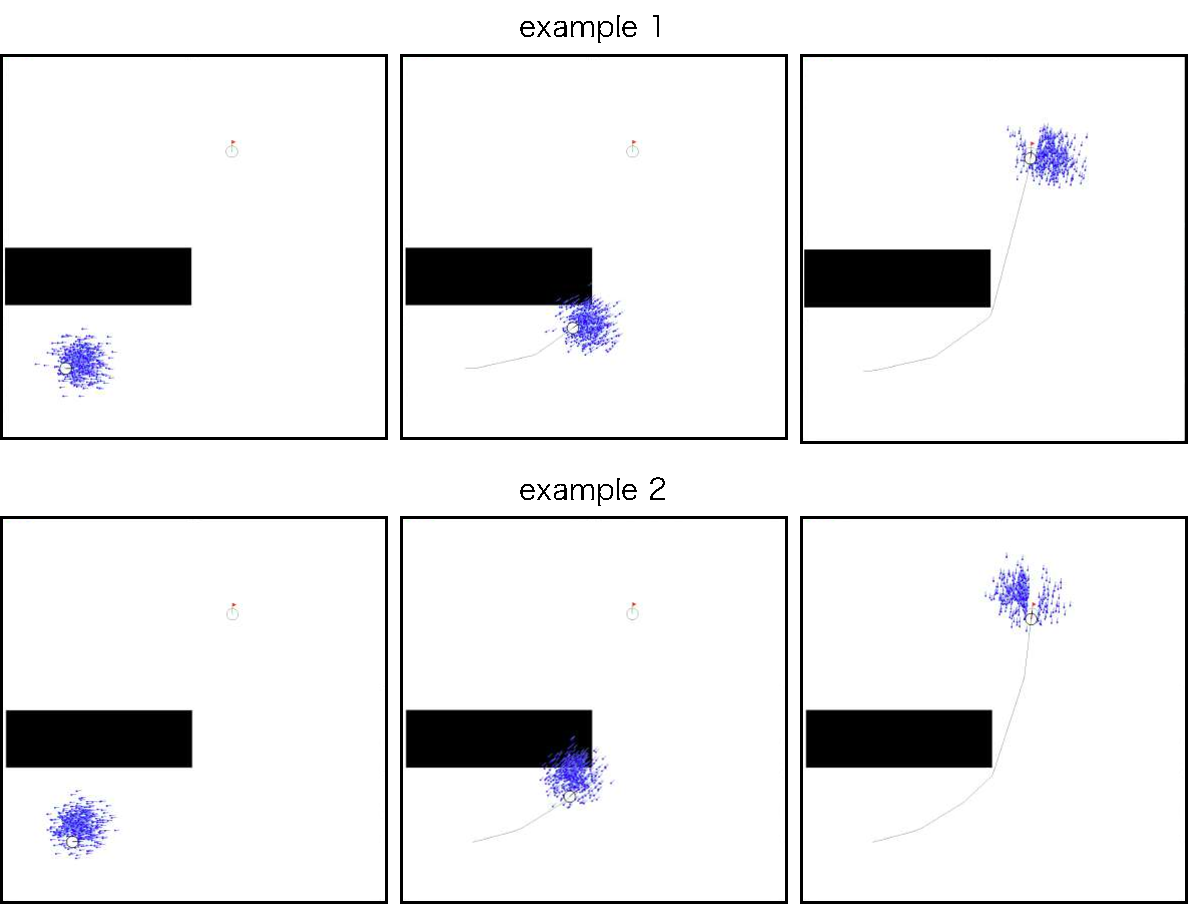
\includegraphics[width=12cm, ]{true_pose.pdf}
    \caption{True pose.}
    \label{fig:true pose}
  \end{center}
\end{figure}

\begin{figure}[tbp]
  \begin{center}
    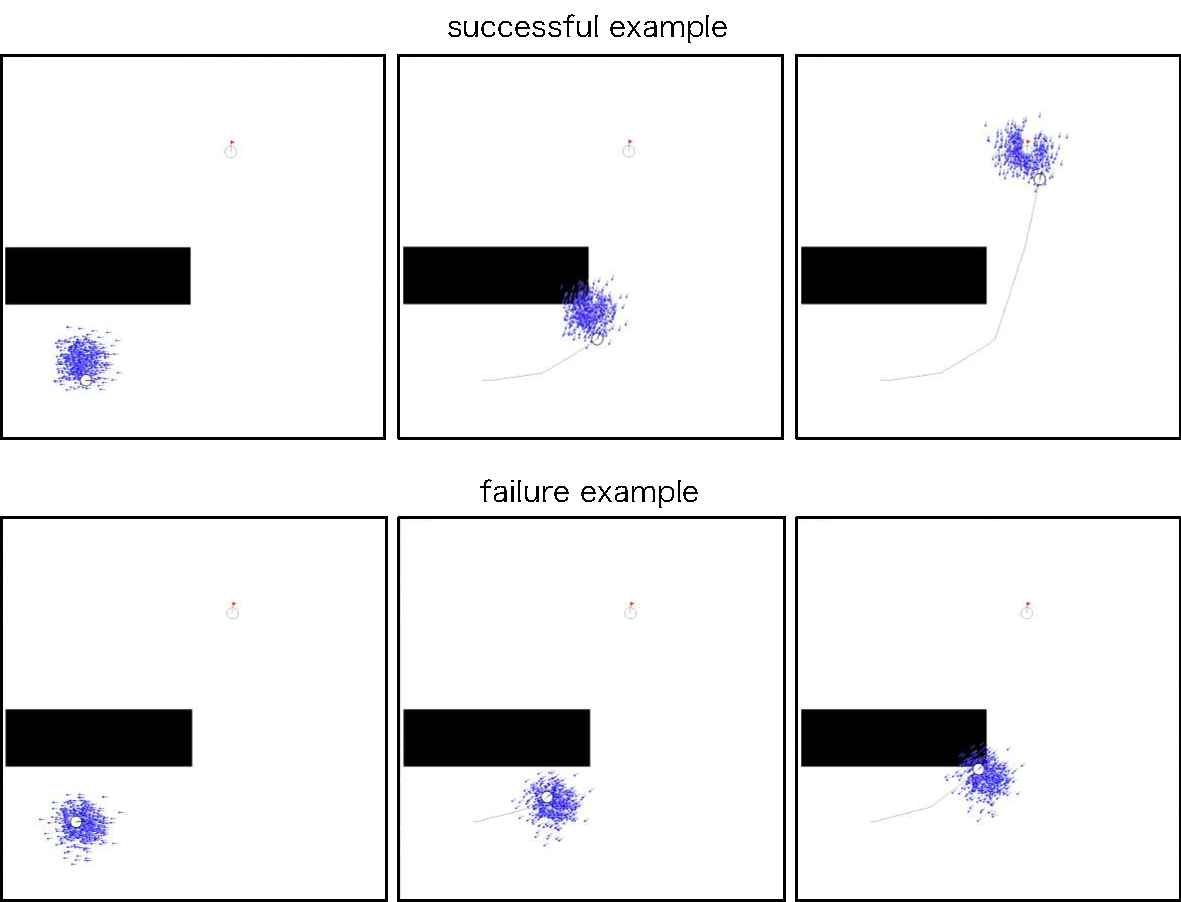
\includegraphics[width=12cm, ]{average_pose.pdf}
    \caption{Average pose of particles.}
    \label{fig:average pose}
  \end{center}
\end{figure}

\begin{figure}[tbp]
  \begin{center}
    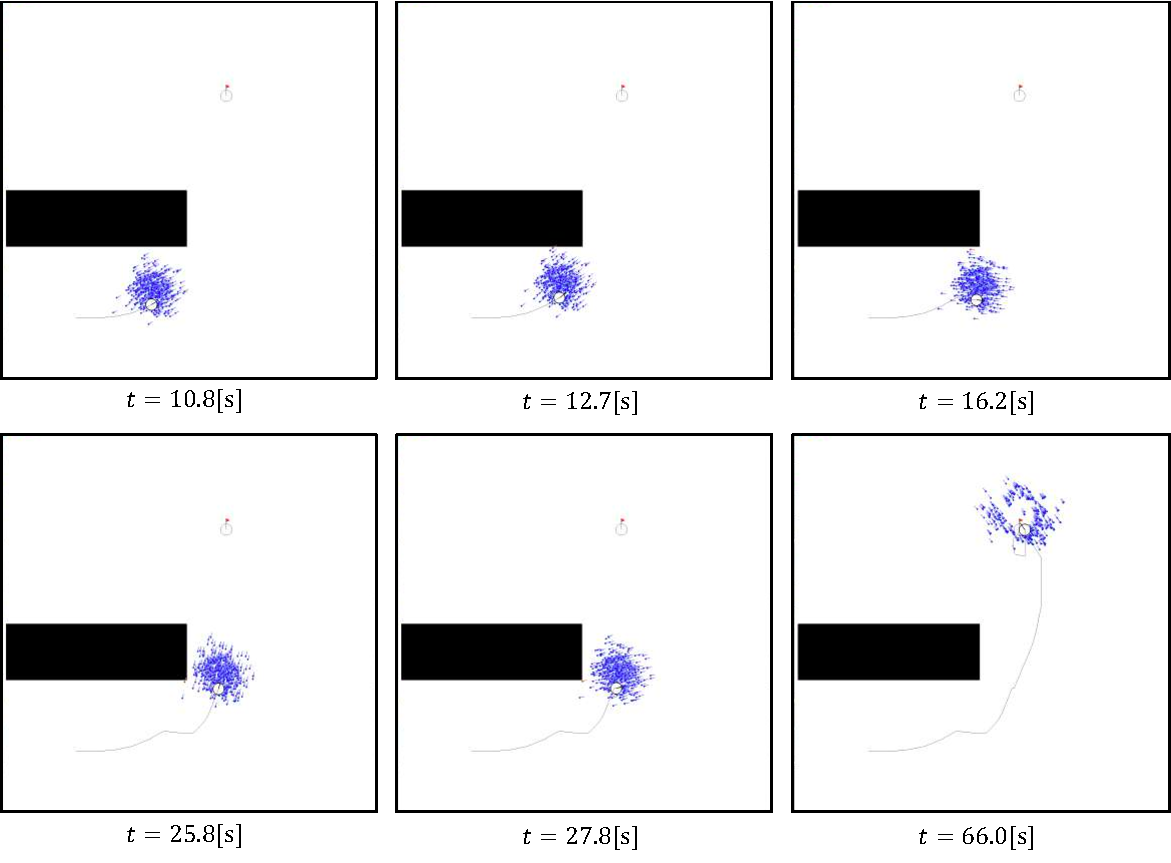
\includegraphics[width=12cm, ]{avoid_pfc_good.pdf}
    \caption{PFC with avoidance good.}
    \label{fig:avoid pfc good}
  \end{center}
\end{figure}

\begin{figure}[tbp]
  \begin{center}
    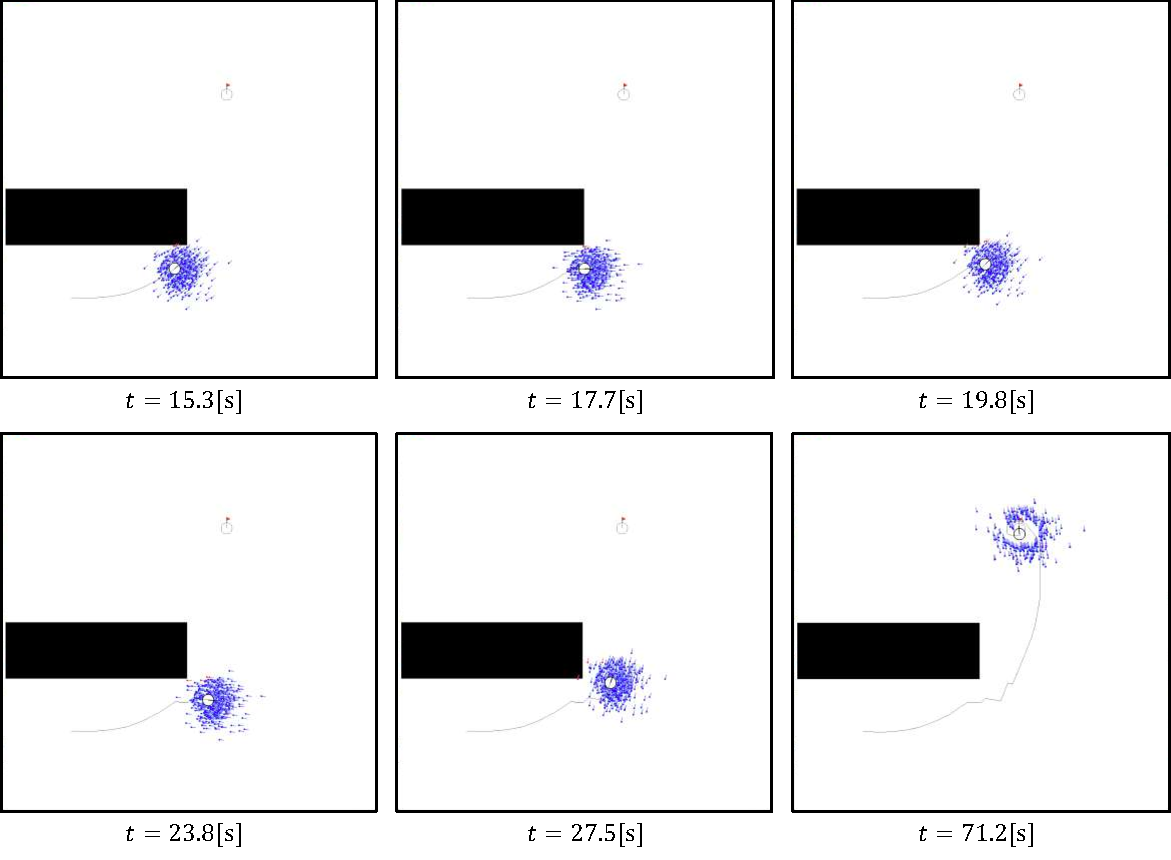
\includegraphics[width=12cm, ]{avoid_pfc_kakukaku.pdf}
    \caption{PFC with avoidance kakukaku.}
    \label{fig:avoid pfc kakukaku}
  \end{center}
\end{figure}

\begin{figure}[tbp]
  \begin{center}
    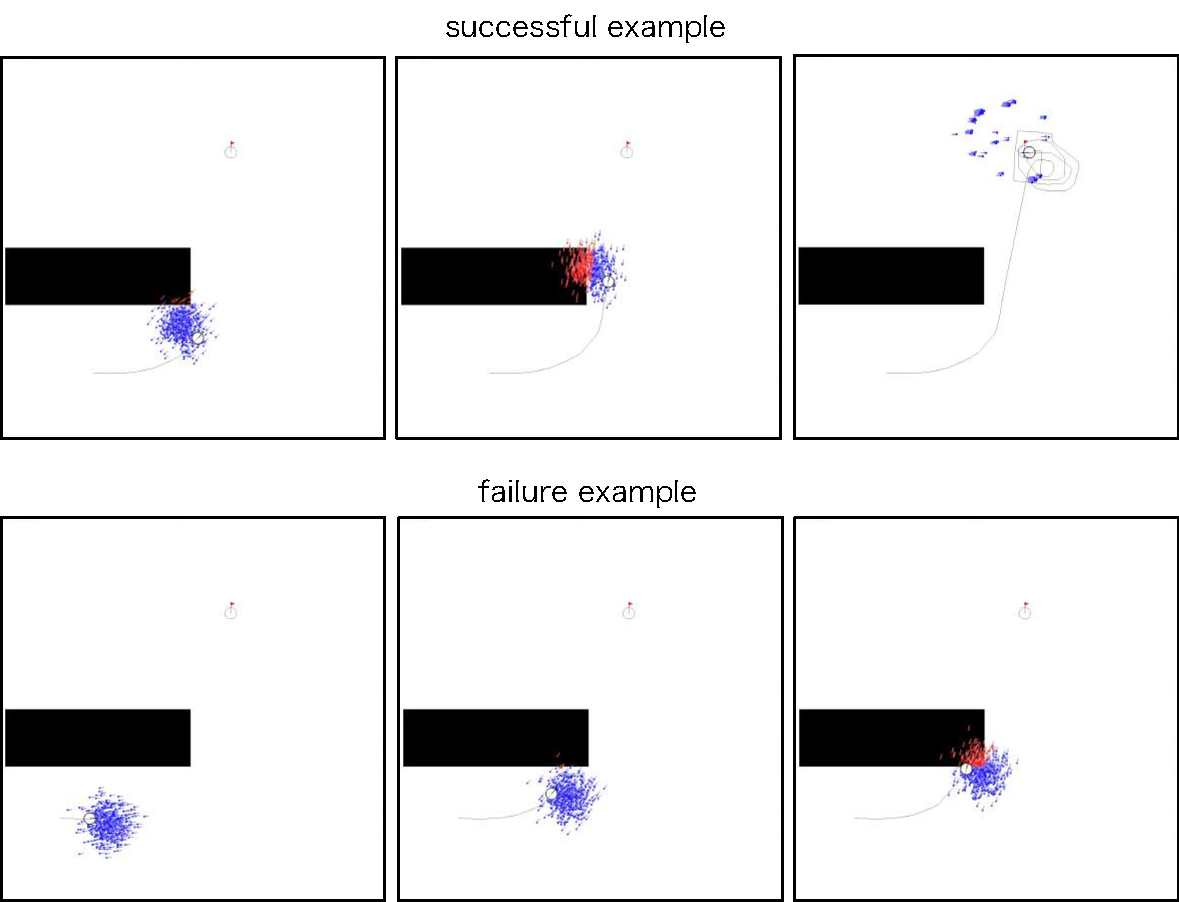
\includegraphics[width=12cm, ]{pfc.pdf}
    \caption{PFC}
    \label{fig:pfc}
  \end{center}
\end{figure}

\begin{figure}[tbp]
  \begin{center}
    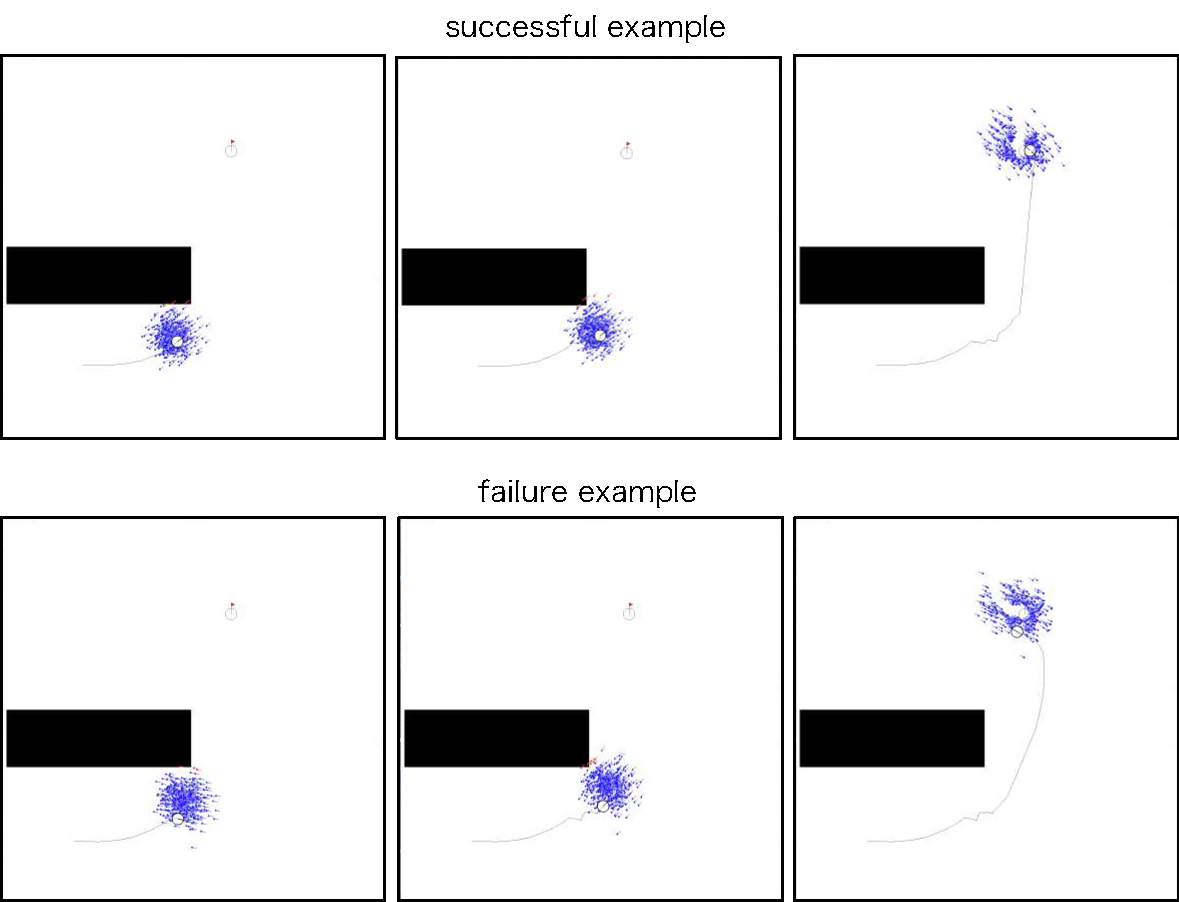
\includegraphics[width=12cm, ]{q-mdp.pdf}
    \caption{Q-MDP}
    \label{fig:q-mdp}
  \end{center}
\end{figure}

%%%%%%%%%%%%%%%%%%%%%%%%%%%%%%%%%%%%%%%%%%%%%%%%%%%%%%%%%%%%%%%%%%%%%%%%%%%%%%%%
% \section{考察} \label{section:考察}
